%% ============================================================
%% AUV Software Documentation -- original architecture description,
%% with the gate return-leg (retracing) added to Section 3.1 and an
%% updated mission map in Section 10.
%% Compile: pdflatex AUV_Software_Documentation_final.tex  (x2)
%% ============================================================
\documentclass[10.5pt,a4paper]{article}

\usepackage[T1]{fontenc}
\usepackage[utf8]{inputenc}
\usepackage{libertinus}
\usepackage{montserrat}
\usepackage{microtype}
\usepackage[margin=1.9cm,top=1.7cm,bottom=1.9cm]{geometry}
\usepackage{graphicx}
\usepackage{xcolor}
\usepackage{amsmath,amssymb}
\usepackage{booktabs}
\usepackage{array}
\usepackage{tabularx}
\usepackage{calc}
\usepackage{colortbl}
\usepackage{enumitem}
\usepackage{listings}
\usepackage{caption}
\captionsetup{labelformat=empty, font=small, skip=4pt}
\usepackage{tikz}
\usetikzlibrary{arrows.meta,positioning,calc,fit}
\usepackage{hyperref}
\usepackage{fancyhdr}
\usepackage{titlesec}
\usepackage{float}
\usepackage[most]{tcolorbox}
\usepackage{setspace}

\definecolor{ink}{HTML}{16233A}
\definecolor{inksoft}{HTML}{4A5568}
\definecolor{accent}{HTML}{6A3FA0}
\definecolor{accentsoft}{HTML}{F1EAFB}
\definecolor{codeorange}{HTML}{F7B267}
\definecolor{codeorangetxt}{HTML}{7A4A00}
\definecolor{hairline}{HTML}{D8DEE6}
\definecolor{tablehead}{HTML}{F3F5F7}
\definecolor{newbg}{HTML}{EAF7EE}
\definecolor{newbd}{HTML}{2E7D32}

\hypersetup{colorlinks=true, linkcolor=accent, urlcolor=accent,
  pdftitle={AUV Software Documentation}, pdfauthor={AUV Team}}

\titleformat{\section}
  {\normalfont\fontfamily{Montserrat-TLF}\selectfont\large\bfseries\color{ink}}
  {\thesection}{0.55em}{}
  [\vspace{1pt}\textcolor{accent}{\rule{\linewidth}{1pt}}\vspace{1pt}]
\titlespacing*{\section}{0pt}{0.9em}{0.45em}
\titleformat{\subsection}
  {\normalfont\fontfamily{Montserrat-TLF}\selectfont\normalsize\bfseries\color{ink}}
  {\thesubsection}{0.55em}{}
\titlespacing*{\subsection}{0pt}{0.7em}{0.3em}
\titleformat{\subsubsection}
  {\normalfont\fontfamily{Montserrat-TLF}\selectfont\small\bfseries\color{inksoft}}
  {}{0em}{}
\titlespacing*{\subsubsection}{0pt}{0.5em}{0.2em}

\pagestyle{fancy}\fancyhf{}
\renewcommand{\headrulewidth}{0pt}
\renewcommand{\footrulewidth}{0.5pt}
\fancyfoot[L]{\footnotesize\color{inksoft}AUV Software Documentation}
\fancyfoot[R]{\footnotesize\color{inksoft}\thepage}

\newcolumntype{C}[1]{>{\centering\arraybackslash}p{#1}}
\newcolumntype{L}[1]{>{\raggedright\arraybackslash}p{#1}}
\renewcommand{\arraystretch}{1.25}
\setlength{\parskip}{3.4pt}
\setlength{\parindent}{0pt}

\newcommand{\hl}[1]{\tikz[baseline=(t.base)]{\node[fill=codeorange,rounded corners=2pt,inner sep=2pt,font=\ttfamily\scriptsize,text=codeorangetxt] (t) {#1};}}
\newcommand{\code}[1]{\texttt{\small\color{accent}#1}}

\tcbuselibrary{skins,breakable}
\newtcolorbox{addedbox}[1][]{colback=newbg, colframe=newbd, coltitle=white,
  boxrule=0.7pt, fonttitle=\fontfamily{Montserrat-TLF}\bfseries\small, title={New in This Revision}, rounded corners,
  left=6pt,right=6pt,top=3pt,bottom=3pt, #1}

\tikzset{
  fsmbox/.style={rectangle,rounded corners=3pt,draw=accent,line width=1pt,
    fill=accentsoft,text=ink,align=center,font=\scriptsize,
    minimum height=0.6cm,text width=3.5cm,inner sep=3pt},
  newfsmbox/.style={rectangle,rounded corners=3pt,draw=newbd,line width=1pt,
    fill=newbg,text=ink,align=center,font=\scriptsize,
    minimum height=0.6cm,text width=3.5cm,inner sep=3pt},
  topobox/.style={rectangle,rounded corners=3pt,draw=accent,line width=0.9pt,
    fill=accentsoft,text=ink,align=center,font=\scriptsize,
    minimum height=0.55cm,text width=2.3cm,inner sep=2.5pt},
  fsmarr/.style={-Stealth,line width=0.9pt,color=ink},
  fsmlabel/.style={font=\tiny\itshape,color=inksoft},
}

\begin{document}

%% ============================================================
\section{Description of Software Architecture}

Our AUV's entire software stack runs on \textbf{ROS 2 (Humble)}. In this upgraded release,
the architecture has evolved from an early prototype into a modular, production-grade
ecosystem. We partitioned the codebase into discrete, decoupled packages -- \hl{auv\_vision},
\hl{auv\_planner}, \hl{auv\_controls}, \hl{auv\_propulsion}, \hl{auv\_sensors}, and
\hl{auv\_telemetry} -- so that high-rate closed-loop propulsion, computer vision inference,
deterministic state-machine planning, and black-box telemetry logging execute independently
without blocking one another. All inter-node communication occurs strictly via asynchronous
ROS 2 topics and standard message interfaces.

The complete software repository is structured within a clean workspace layout shown below:

\begin{figure}[H]
\centering
\begin{lstlisting}[basicstyle=\ttfamily\scriptsize,frame=single,framesep=5pt,
  rulecolor=\color{hairline},backgroundcolor=\color{tablehead},breaklines=true]
auv_ws/src/
|-- auv_bringup/
|   |-- launch/ (sim_mission.launch.py, bridge.launch.py)
|   `-- config/ (sim_params.yaml, real_params.yaml)
|-- auv_vision/
|   |-- gate_detector_node.py
|   |-- gate_localizer_node.py
|   |-- blue_bin_detector_node.py
|   |-- blue_bin_cv_detector_node.py
|   |-- blue_bin_localizer_node.py
|   |-- green_detector_node.py
|   |-- green_localizer_node.py
|   |-- red_bin_detector_node.py
|   |-- red_bin_localizer_node.py
|   |-- qr_detector_node.py
|   |-- qr_localizer_node.py
|   `-- underwater_view_node.py
|-- auv_planner/
|   |-- gate_navigator_v2_node.py
|   `-- green_navigator_node.py
|-- auv_controls/
|   `-- velocity_controller_node.py
|-- auv_propulsion/
|   `-- thruster_allocator_node.py
|-- auv_sensors/
|   |-- launch/ (state_estimation.launch.py)
|   `-- config/ (ekf.yaml)
`-- auv_telemetry/
    |-- mission_logger_node.py
    |-- mission_monitor_node.py
    `-- trail_mapper_node.py
\end{lstlisting}
\caption{Fig 1. High-Level Software Architecture \& ROS 2 Package Organization}
\end{figure}

Rather than reviewing folders in isolation, the specific responsibilities, node
architectures, and topic flows of each package are detailed organically alongside the
respective vehicle functionalities in the sections that follow.

%% ============================================================
\section{Salient Features of the Software Stack}

\begin{itemize}[leftmargin=1.3em,itemsep=2pt]
  \item \textbf{Closed-Loop Physics Simulation \& 8-Thruster Allocation
    (\hl{auv\_controls} \& \hl{auv\_propulsion}):} Rather than perfectly tracking velocity
    commands via kinematic teleportation, the AUV is driven by 8 simulated physical
    thrusters. A closed-loop P-controller continuously calculates restorative body wrenches,
    which are translated into individual thruster forces via a Moore-Penrose pseudo-inverse
    allocation matrix.
  \item \textbf{Stereo-Vision Based 3D Localization (\hl{auv\_vision}):} Instead of relying
    on acoustic sensors, we compute 3D gate/bin coordinates by correlating YOLO bounding
    boxes with stereo disparity maps. The localizer interrogates four prioritized geometric
    candidate points across a 9$\times$9 disparity patch, taking the median of valid pixels
    to apply the standard \code{depth = fx * baseline / disparity} formula with a
    plausibility guard (0.2m--19.1m).
  \item \textbf{Dual-Camera Cross-Handoff:} The front stereo camera pair handles long-range
    acquisition and approach. The downward-facing camera takes over once the AUV is directly
    above a target, using odometry-based altitude for pinhole projection instead of stereo
    disparity. The system transitions seamlessly between them based on target coverage.
  \item \textbf{Dead-Reckoning Visual Fallback (\hl{auv\_planner}):} When targets exit the
    camera field-of-view during terminal approach, the navigators switch smoothly from live
    YOLO tracking to odometry dead-reckoning using the last verified target coordinates in
    the global odom frame, maintaining trajectory stability.
  \item \textbf{HSV-Based False-Positive Reduction:} For the bottom camera's blue-bin task,
    we built \hl{blue\_bin\_cv\_detector\_node} which only accepts a blue blob if at least
    15\% of its pixel area spatially overlaps the green mat in the same frame. Open blue
    water structurally cannot pass this check, eliminating false positives without needing
    additional neural network training data.
  \item \textbf{Active Safety Envelope \& Wall Repulsion:} The controller actively damps
    roll and pitch oscillations via restoring torque if tilt exceeds 35\textdegree, enforces
    a safe depth envelope ($-$8.0m to +3.0m), and applies repulsive potential forces
    (300 N/m) when within 1.0m of any pool boundary.
  \item \textbf{Post-Mission Trail Mapping \& Live Dashboard (\hl{auv\_telemetry}):} The
    \hl{trail\_mapper\_node} records the AUV's trajectory every 0.1m, renders it as a
    colour-coded mission-progress plot with true-to-scale gate/bin/mat footprints on the
    pool boundary, and exports interactive 3D HTML maps, while \hl{mission\_monitor\_node}
    provides a real-time ANSI terminal dashboard.
\end{itemize}

%% ============================================================
\section{Logical Steps in the Working of Software Components}

Mission planning is managed inside the \hl{auv\_planner} package by two coordinating finite
state machine nodes: \hl{gate\_navigator\_v2\_node} for initial arena traversal and
\hl{green\_navigator\_node} for post-gate target centering.

\subsection{Gate Navigation (\texttt{gate\_navigator\_v2\_node})}

The gate navigator is a deliberately simplified \emph{one-pass} FSM -- it crosses the gate once
and hands off immediately, with no U-turn or return leg of its own (that return trip is now
part of the post-gate mission instead; see Step 5 in Section~3.2).

\textbf{STEP 1: FORWARD DRIVE} -- When \code{sim\_mission.launch.py} starts, the gate
navigator begins in the FORWARD state. It drives straight ahead at 0.20 m/s for 3.5 metres
using pure odometry. If the YOLO detector spots the gate during this phase, it skips directly
to TRACK.

\textbf{STEP 2: LATERAL SEARCH} -- If the gate was not acquired during the forward phase, the
AUV enters SEARCH. It strafes sideways at 0.15 m/s, sweeping $\pm$6.0 metres from its center
position while holding heading with a P-controller until a confident gate detection is
registered.

\textbf{STEP 3: TRACK AND APPROACH} -- In TRACK, the AUV drives toward a staging point 1.5m
in front of the gate at up to 0.15 m/s while correcting its heading using the bearing error to
the gate's odom-frame coordinates. If the YOLO feed goes stale (older than 1.5 seconds), it
falls back to odom dead-reckoning to the last known position.

\textbf{STEP 4: COMMIT, ALIGN, AND CROSS} -- Once within 0.5m of the staging point, the AUV
locks its approach heading and enters ALIGN. It rotates in place until the yaw error drops
below 0.05 rad (2.86\textdegree) for 8 consecutive ticks, then enters CROSS -- driving
straight through the gate with a 3.25m overshoot to clear the structure entirely, then
publishes state \texttt{"DONE"} and hands off directly to \texttt{green\_navigator\_node}.

\begin{figure}[H]\centering
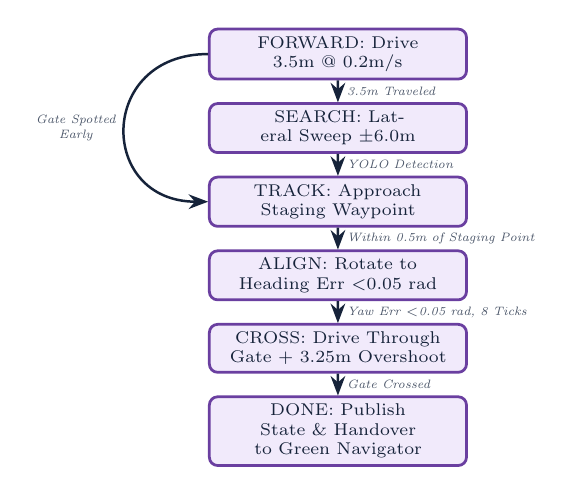
\begin{tikzpicture}[scale=0.88, every node/.append style={scale=0.88}, node distance=0.28cm and 1.5cm]
  \node[fsmbox] (fwd)  {FORWARD: Drive 3.5m @ 0.2m/s};
  \node[fsmbox, below=of fwd] (srch) {SEARCH: Lateral Sweep $\pm$6.0m};
  \node[fsmbox, below=of srch] (trk) {TRACK: Approach Staging Waypoint};
  \node[fsmbox, below=of trk] (aln) {ALIGN: Rotate to Heading Err $<$0.05 rad};
  \node[fsmbox, below=of aln] (crs) {CROSS: Drive Through Gate + 3.25m Overshoot};
  \node[fsmbox, below=of crs] (done) {DONE: Publish State \& Handover to Green Navigator};

  \draw[fsmarr] (fwd) -- (srch) node[midway,right,fsmlabel]{3.5m Traveled};
  \draw[fsmarr] (srch) -- (trk) node[midway,right,fsmlabel]{YOLO Detection};
  \draw[fsmarr] (trk) -- (aln) node[midway,right,fsmlabel]{Within 0.5m of Staging Point};
  \draw[fsmarr] (aln) -- (crs) node[midway,right,fsmlabel]{Yaw Err $<$0.05 rad, 8 Ticks};
  \draw[fsmarr] (crs) -- (done) node[midway,right,fsmlabel]{Gate Crossed};
  \draw[fsmarr] (fwd.west) .. controls +(-1.6,0) and +(-1.6,0) .. (trk.west)
    node[midway,left,fsmlabel,align=center]{Gate Spotted\\Early};
\end{tikzpicture}
\caption{Fig 2. Gate Navigator State Machine (\texttt{auv\_planner/gate\_navigator\_v2\_node}) -- one-pass only, no return leg.}
\end{figure}

\subsection{Post-Gate Navigation (\texttt{green\_navigator\_node})}

After the gate navigator publishes \texttt{"DONE"}, the \hl{green\_navigator\_node} takes
over through an automated multi-stage sequence covering the green mat, blue bin, payload
drop, and -- as of this revision -- the full trip back to the start point:

\begin{enumerate}[leftmargin=1.6em,itemsep=1pt]
  \item \textbf{CLEAR\_GATE:} Drives straight forward 0.46m (about half the AUV's length)
    immediately upon handover, opening clearance from the gate posts before any yaw turn.
  \item \textbf{RESET\_YAW:} Snaps heading back to the locked reference yaw published on
    \code{/auv/forward\_reference\_yaw} (the heading at mission start) -- used again before
    the bin search so every lateral sweep below scans facing dead-ahead.
  \item \textbf{SEARCH\_GREEN:} Advance-and-sweep search for the green mat: strafes
    $\pm$20.0m at 0.25 m/s, left first, creeping 3.0m forward per full pass up to a 15.0m
    total advance budget. If the mat is never found, skips straight to RISE\_FOR\_SURVEY
    rather than stalling, since blue-bin YOLO detection is reliable on its own.
  \item \textbf{APPROACH\_GREEN:} Drives toward the green mat's odom coordinate until bottom
    -camera coverage, a front-camera on-mat sighting, or 2.0m proximity confirms it is over
    the zone.
  \item \textbf{RISE\_FOR\_SURVEY:} Climbs exactly one robot-height (0.58m, taken from the
    AUV's own collision geometry) above its green-zone cruising depth, then RESET\_YAW again
    before the bin search.
  \item \textbf{SEARCH\_BLUE\_BIN:} Tighter sweep ($\pm$3.0m, 8.0m advance budget) for the
    blue bin. If this budget is exhausted, the FSM falls back to an identical
    SEARCH\_RED\_BIN $\to$ APPROACH\_RED\_BIN $\to$ RISE\_FOR\_VERIFICATION\_RED $\to$
    CENTER\_RED\_BIN sequence for the red bin instead, tagging the eventual HOLD target as
    ``red'' rather than ``blue''.
  \item \textbf{APPROACH\_BLUE\_BIN \& RISE\_FOR\_VERIFICATION:} Drives to the stored bin
    coordinate, tapering speed on approach, then rises $\sim$0.5m for a wider bottom-camera
    view once within 0.35m or directly overhead.
  \item \textbf{CENTER\_BLUE\_BIN \& HOLD:} Bottom-camera visual servoing fine-centers the
    drum, requiring the error to stay under 0.35m for 10 consecutive ticks with the green mat
    confirmed underneath; the vehicle then holds position for 5 seconds.
\end{enumerate}

\begin{addedbox}
\textbf{STEP 5: PAYLOAD DROP \& RETURN LEG} -- Reaching the blue bin's HOLD state no longer
ends the mission: the payload is released there, and the AUV then retraces its own path all
the way back to the start point.
\begin{itemize}[leftmargin=1.2em,itemsep=1pt,topsep=2pt]
  \item \textbf{DESCEND\_TO\_BIN} -- eases down half a robot-height below the HOLD altitude
    (only when the held target is the \emph{blue} bin -- a red-bin-only HOLD skips this and
    the drop, going straight to SURFACE\_AND\_TURN, since the payload only ever releases on
    the blue bin).
  \item \textbf{DROP\_PAYLOAD} -- holds position for 3 seconds while the payload releases.
  \item \textbf{SURFACE\_AND\_TURN} -- builds the return route from the AUV's own recorded
    trail, reversed and downsampled to $\sim$0.5m spacing with the lateral search sweeps
    excluded (so the outbound zig-zag isn't replayed), then climbs back to the HOLD altitude
    and turns to face the first return waypoint.
  \item \textbf{RETRACE\_PATH} -- flies the reversed waypoint sequence, holding the same
    altitude the outbound trail recorded at each point (rather than a fixed cruise height) so
    it clears the gate structure on the way back, then publishes state \texttt{"FINAL\_DONE"}
    once the start zone is reached.
\end{itemize}
This return leg replaces what earlier revisions of this document described as a gate-level
U-turn: the AUV now retraces its own dead-reckoned trail across the \emph{entire} mission
(gate, green zone, and bin) rather than re-detecting and re-crossing just the gate.
\end{addedbox}

\begin{figure}[H]\centering
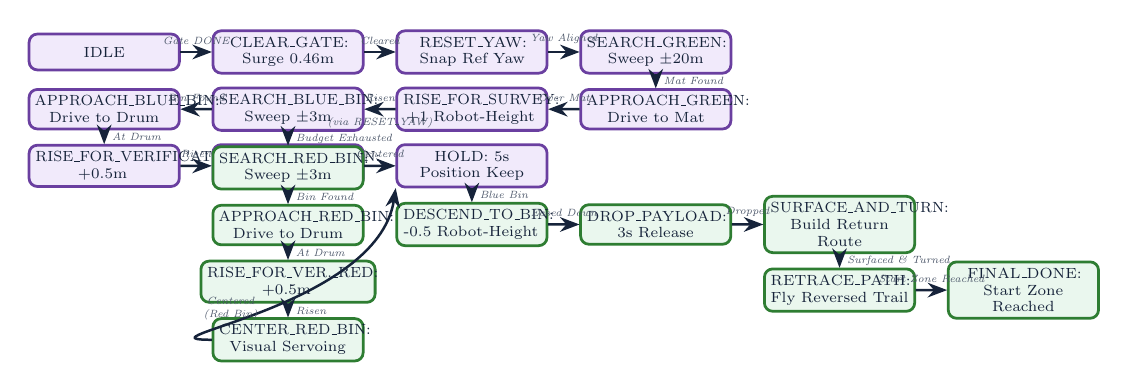
\begin{tikzpicture}[scale=0.76, every node/.append style={scale=0.76}, node distance=0.18cm and 0.4cm]
  \node[fsmbox,text width=2.3cm] (idle) {IDLE};
  \node[fsmbox,text width=2.3cm,right=of idle] (cg) {CLEAR\_GATE: Surge 0.46m};
  \node[fsmbox,text width=2.3cm,right=of cg] (ry) {RESET\_YAW: Snap Ref Yaw};
  \node[fsmbox,text width=2.3cm,right=of ry] (sg) {SEARCH\_GREEN: Sweep $\pm$20m};
  \node[fsmbox,text width=2.3cm, below=of sg] (ag) {APPROACH\_GREEN: Drive to Mat};
  \node[fsmbox,text width=2.3cm, left=of ag] (rfs) {RISE\_FOR\_SURVEY: +1 Robot-Height};
  \node[fsmbox,text width=2.3cm, left=of rfs] (sb) {SEARCH\_BLUE\_BIN: Sweep $\pm$3m};
  \node[fsmbox,text width=2.3cm, left=of sb] (ab) {APPROACH\_BLUE\_BIN: Drive to Drum};
  \node[fsmbox,text width=2.3cm, below=of ab] (rfv) {RISE\_FOR\_VERIFICATION: +0.5m};
  \node[fsmbox,text width=2.3cm, right=of rfv] (cb) {CENTER\_BLUE\_BIN: Visual Servoing};
  \node[fsmbox,text width=2.3cm, right=of cb] (hold) {HOLD: 5s Position Keep};
  \node[newfsmbox,text width=2.3cm, below=of hold] (dtb) {DESCEND\_TO\_BIN: -0.5 Robot-Height};
  \node[newfsmbox,text width=2.3cm, right=of dtb] (dp) {DROP\_PAYLOAD: 3s Release};
  \node[newfsmbox,text width=2.3cm, right=of dp] (sat) {SURFACE\_AND\_TURN: Build Return Route};
  \node[newfsmbox,text width=2.3cm, below=of sat] (rp) {RETRACE\_PATH: Fly Reversed Trail};
  \node[newfsmbox,text width=2.3cm, right=of rp] (fd) {FINAL\_DONE: Start Zone Reached};

  \node[newfsmbox,text width=2.3cm, below=of sb] (srb) {SEARCH\_RED\_BIN: Sweep $\pm$3m};
  \node[newfsmbox,text width=2.3cm, below=of srb] (arb) {APPROACH\_RED\_BIN: Drive to Drum};
  \node[newfsmbox,text width=2.7cm, below=of arb] (rfvr) {RISE\_FOR\_VER.\_RED: +0.5m};
  \node[newfsmbox,text width=2.3cm, below=of rfvr] (crb) {CENTER\_RED\_BIN: Visual Servoing};

  \draw[fsmarr] (idle) -- (cg) node[midway,above,fsmlabel]{Gate DONE};
  \draw[fsmarr] (cg) -- (ry) node[midway,above,fsmlabel]{Cleared};
  \draw[fsmarr] (ry) -- (sg) node[midway,above,fsmlabel]{Yaw Aligned};
  \draw[fsmarr] (sg) -- (ag) node[midway,right,fsmlabel]{Mat Found};
  \draw[fsmarr] (ag) -- (rfs) node[midway,above,fsmlabel]{Over Mat};
  \draw[fsmarr] (rfs) -- (sb) node[midway,above,fsmlabel]{Risen}
    node[midway,below,fsmlabel]{(via RESET\_YAW)};
  \draw[fsmarr] (sb) -- (ab) node[midway,above,fsmlabel]{Bin Found};
  \draw[fsmarr] (ab) -- (rfv) node[midway,right,fsmlabel]{At Drum};
  \draw[fsmarr] (rfv) -- (cb) node[midway,above,fsmlabel]{Risen};
  \draw[fsmarr] (cb) -- (hold) node[midway,above,fsmlabel]{Centered};
  \draw[fsmarr] (hold) -- (dtb) node[midway,right,fsmlabel]{Blue Bin};
  \draw[fsmarr] (dtb) -- (dp) node[midway,above,fsmlabel]{Eased Down};
  \draw[fsmarr] (dp) -- (sat) node[midway,above,fsmlabel]{Dropped};
  \draw[fsmarr] (sat) -- (rp) node[midway,right,fsmlabel]{Surfaced \& Turned};
  \draw[fsmarr] (rp) -- (fd) node[midway,above,fsmlabel]{Start Zone Reached};

  \draw[fsmarr] (sb) -- (srb) node[midway,right,fsmlabel]{Budget Exhausted};
  \draw[fsmarr] (srb) -- (arb) node[midway,right,fsmlabel]{Bin Found};
  \draw[fsmarr] (arb) -- (rfvr) node[midway,right,fsmlabel]{At Drum};
  \draw[fsmarr] (rfvr) -- (crb) node[midway,right,fsmlabel]{Risen};
  \draw[fsmarr] (crb.west) .. controls +(-1.4,0) and +(-0.3,-2.0) .. (hold.south west)
    node[midway,left,fsmlabel,align=center]{Centered\\(Red Bin)};
\end{tikzpicture}
\caption{Fig 3. Post-Gate Navigator State Machine (\texttt{auv\_planner/green\_navigator\_node}) -- extended with the red-bin fallback and the payload-drop/return-leg states (highlighted).}
\end{figure}

%% ============================================================
\section{Dataset Preparation and Object Classes}

Building a reliable underwater object detection system meant we needed training data that
accurately matched what our cameras see. Off-the-shelf datasets lack the competition arena's
custom PVC gate dimensions, colored drums, and floor target mats, requiring a tailored
dataset synthesis.

\subsection{Data Sources}

\textbf{Simulation-Generated Images:} We set up the full competition arena in Gazebo
Harmonic using SDF world models (PVC gate, 8m$\times$2m green target mat, blue drum, 3 red
drums, colored flares, and QR-coded boxes). To capture comprehensive viewpoints, we developed
an automated test harness (\hl{bottom\_cam\_altitude\_test.py}) that systematically teleports
the AUV across a coordinate grid over arena elements at 5 altitudes and 6 lateral offsets,
capturing thousands of annotated training frames across varied viewing angles and distances.

\textbf{Kaggle and External Sources:} To reduce simulation overfitting, we supplemented our
captures with underwater imagery from Kaggle datasets. These introduced natural variations in
water turbidity, suspended particle backscatter, and dynamic lighting conditions.

\subsection{Object Classes in the Dataset}

\begin{table}[H]\centering\small
\begin{tabularx}{\textwidth}{L{2.2cm} X L{4.6cm}}
\toprule
\rowcolor{tablehead}\textbf{Class} & \textbf{Description \& Arena Physical Geometry} & \textbf{Detection \& Localization Modality} \\
\midrule
Gate & Two vertical PVC posts with a connecting crossbar; 1.5m passage width & YOLOv8n + 4-Candidate Stereo Disparity \\
Blue Bin & Blue cylindrical drum (0.3m radius, 0.5m height) positioned on green mat & YOLOv8n (Front) + HSV Green-Overlap (Bottom) \\
Red Bin & Red cylindrical drums (same dimensions as blue); 3 placed on target mat & YOLOv8n + Altitude Pinhole Projection \\
QR Code & 0.5m $\times$ 0.5m target cube with encoded mission payload markers on pool floor & OpenCV QRCodeDetector + Altitude Projection \\
Flares & Colored cylinders (orange, blue, red, yellow) placed at mid-water depth & YOLOv8n Bounding Box Inference \\
Green Target Mat & 8m $\times$ 2m flat mat on pool floor; acts as landing zone for the bin task & Classical HSV Color Segmentation \\
\bottomrule
\end{tabularx}
\end{table}

\subsection{Model Details}

We use YOLOv8n (nano) as our detection backbone, providing the ideal balance of inference
latency (45 FPS onboard) and mAP. For the green target mat, we skip neural inference
entirely and use classical HSV color thresholding with morphological cleanup, which is
lighter, faster, and immune to neural false positives. For the bottom camera's blue bin task,
\hl{blue\_bin\_cv\_detector\_node} verifies spatial overlap with the green mat, eliminating
background blue-water triggers.

\begin{figure}[H]\centering
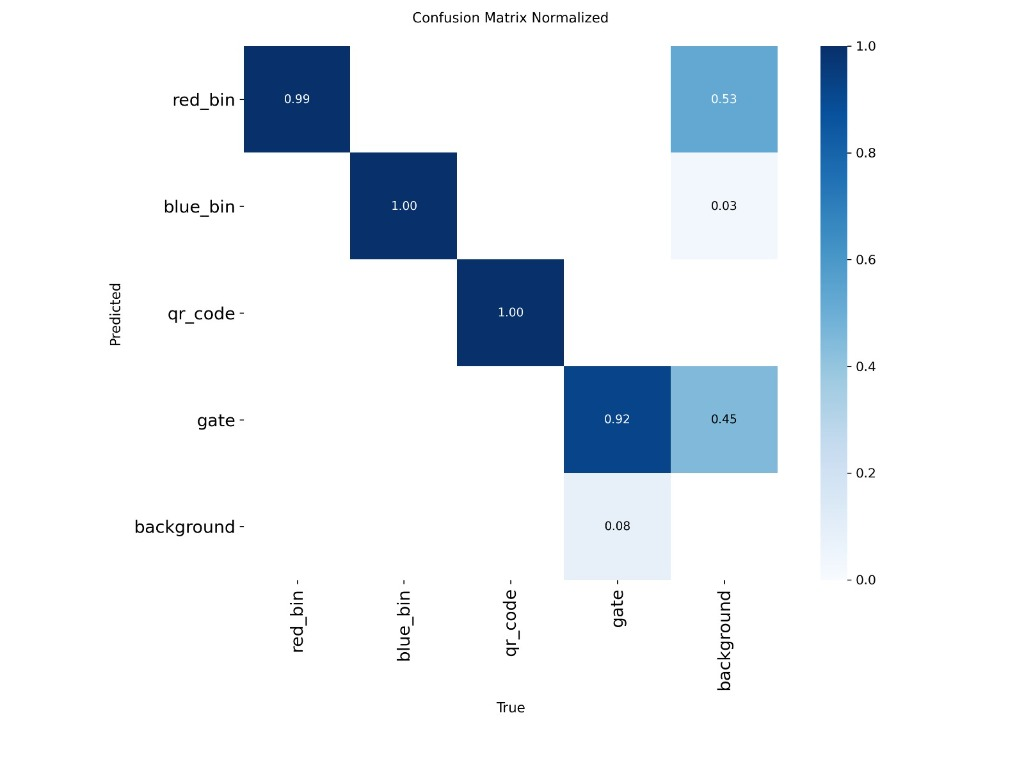
\includegraphics[width=0.5\textwidth]{photos_v2/fig4_confusion_matrix.jpg}\\[2pt]
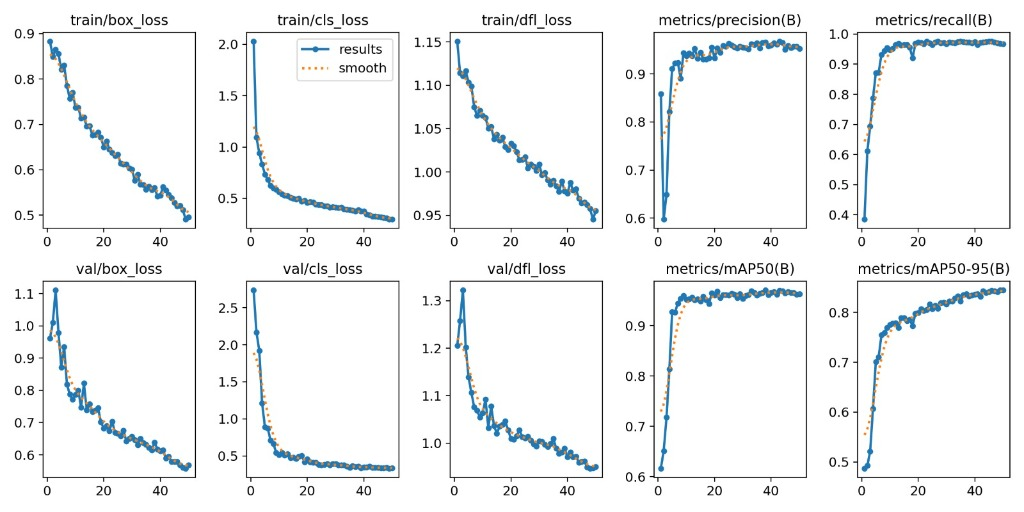
\includegraphics[width=0.92\textwidth]{photos_v2/fig5_training_metrics.jpg}
\caption{Fig 4/5. YOLOv8n Training Confusion Matrix (Normalized Across Arena Classes) and
Training Performance Metrics (Loss Curves, Precision-Recall \& mAP@0.5 Convergence).}
\end{figure}

%% ============================================================
\section{Object Detection and Vision Pipeline}

All perception nodes reside within the \hl{auv\_vision} package. The vision architecture
divides perception into front stereo long-range estimation and downward monocular precision
tracking:

\subsection{Gate Detection Pipeline}

The \hl{gate\_detector\_node} subscribes to the left camera feed
(\code{/model/auv\_box/stereo\_front/left/image\_raw}). Frames are converted via CvBridge to
OpenCV BGR arrays and processed through YOLOv8n (confidence threshold 0.10). The
highest-confidence bounding box is published as a \code{Float32MultiArray} to
\code{/auv/gate\_detection\_2d}.

The \hl{gate\_localizer\_node} fuses this 2D detection with disparity maps from
\code{stereo\_image\_proc}. Because bounding-box centers on a gate frame represent empty
water, the localizer samples four geometric candidate points in priority order: Left Pole
$\to$ Right Pole $\to$ Crossbar $\to$ Center. At each point, it interrogates a 9$\times$9
disparity patch, accepts the first location with $\ge$3 valid pixels, computes the median
disparity $d$, and calculates 3D coordinates:

\begin{center}
$Z_{depth} = (f_x \cdot B) / d, \quad X = (u - c_x)\cdot Z_{depth} / f_x, \quad Y = (v - c_y)\cdot Z_{depth} / f_y \quad (B = 0.075\text{m})$
\end{center}

The resulting metric body position $[x, y, z, \text{conf}]$ is published to
\code{/auv/gate\_position\_3d}.

\subsection{Blue Bin Detection Pipeline}

On the front camera, \hl{blue\_bin\_detector\_node} executes YOLOv8n inference. On the
downward camera, \hl{blue\_bin\_cv\_detector\_node} provides a robust classical fallback. It
creates independent HSV green and blue masks, isolates blue contours, and calculates the
intersection between each blue contour and the dilated green mat mask. A detection is only
published to \code{/auv/blue\_bin\_detection\_bottom\_2d} if at least 15\% of the blue blob
area overlaps the green mat, guaranteeing that open water never triggers a false positive.

\subsection{Green Mat Detection Pipeline}

The \hl{green\_detector\_node} applies HSV segmentation ($H{:}38\text{--}82$,
$S{:}80\text{--}255$, $V{:}60\text{--}255$) with morphological opening and closing. On the
front camera, processing is confined to the lower 40\% region of interest (ROI) because the
floor mat only appears in the bottom portion of the horizontal field-of-view, discarding
surface reflections. The downward camera evaluates the full frame to report coverage area and
metric offset.

\subsection{Red Bin, QR Code \& Underwater View Rendering}

The \hl{red\_bin\_localizer\_node} and \hl{qr\_localizer\_node} project downward camera pixel
coordinates into metric arena coordinates using odometric altitude:
$X = (u - c_x)\cdot h / f_x$, $Y = (v - c_y)\cdot h / f_y$. The \hl{qr\_detector\_node} decodes
floor QR markers using OpenCV's \code{QRCodeDetector} and publishes strings to
\code{/auv/qr\_payload}. In parallel, \hl{underwater\_view\_node} simulates Beer-Lambert
optical attenuation ($I_\lambda = I_0 e^{-\alpha_\lambda z}$) on an isolated output topic for
live visualization.

%% ============================================================
\section{Controls, Propulsion \& Thruster Allocation}

Vehicle movement and hydrodynamic stabilization are managed collaboratively by
\hl{auv\_controls} and \hl{auv\_propulsion}, bridging high-level planner velocity commands to
physical thrusters:

\subsection{8-Thruster Overactuated Geometry}

The AUV features 8 brushless thrusters configured for full 6-DOF overactuated control.
Thrusters $T_1\dots T_4$ are mounted horizontally at $\pm$45\textdegree{} angles relative to
the hull's longitudinal axis, providing decoupled surge ($F_x$), sway ($F_y$), and yaw
($M_z$). Thrusters $T_5\dots T_8$ are positioned vertically at the hull corners, providing
heave ($F_z$), roll ($M_x$), and pitch ($M_y$).

\subsection{Thruster Allocation Matrix (TAM) \& Pseudo-Inverse}

The relationship between desired body wrench $\boldsymbol{\tau} = [F_x, F_y, F_z, M_x, M_y,
M_z]^T$ and individual thruster thrusts $\mathbf{u} = [u_1, \dots, u_8]^T$ is governed by the
thruster geometry matrix $\boldsymbol{\tau} = \mathbf{B}\mathbf{u}$. The
\hl{thruster\_allocator\_node} solves for the optimal, minimum-energy thrust allocation using
the Moore-Penrose pseudo-inverse:

\begin{center}
\small $u = B^T(BB^T)^{-1}\tau \;\Rightarrow\; u_{horiz} = B_H^{+}[F_x,F_y,M_z]^T,\quad u_{vert} = B_V^{+}[F_z,M_x,M_y]^T$
\end{center}

Individual forces are clamped to [$-$40N, +40N] and published to
\code{/model/auv\_box/joint/T\_\{1..8\}/cmd\_thrust}.

\subsection{Closed-Loop Velocity Controller \& Pose Differentiator}

The \hl{velocity\_controller\_node} consumes body velocity commands
(\code{/model/auv\_box/cmd\_vel}) from navigators and compares them against vehicle
velocities. To overcome Gazebo bridge limitations where twist messages in body frames are
unpopulated, the node computes actual velocity via backward finite-differencing on odometry
positions, smoothed by an Exponential Moving Average (EMA) filter ($\alpha = 0.3$):

\begin{center}
\small $v_{raw}[k] = (p[k]-p[k-1])/dt, \quad v_{filt}[k] = \alpha\, v_{raw}[k] + (1-\alpha)\,v_{filt}[k-1]$
\end{center}

Proportional control loops generate the required body wrench: $F_x =
K_{p,x}(v_{x,cmd}-v_{x,filt})$, $F_y = K_{p,y}(v_{y,cmd}-v_{y,filt})$, and $M_z =
K_{p,yaw}(\omega_{z,cmd}-\omega_{z,filt})$, published to \code{/auv/wrench\_cmd}.

\subsection{Triple-Layer Active Safety Envelope}

\begin{itemize}[leftmargin=1.3em,itemsep=2pt]
  \item \textbf{Tipping Damping:} If roll ($|\phi|$) or pitch ($|\theta|$) exceeds
    35\textdegree, the controller damps horizontal forces and commands restorative moments
    ($M_x = -35\phi$, $M_y = -35\theta$) to prevent capsizing.
  \item \textbf{Depth Envelope:} Enforces a hard operational depth envelope between
    $-$8.0m and +3.0m.
  \item \textbf{Pool Wall Repulsion:} When the vehicle approaches within 1.0m of any pool
    perimeter boundary, a continuous repulsive force $F_{rep} = 300\times(1.0-d_{wall})$ N
    pushes the hull away from the wall.
\end{itemize}

%% ============================================================
\section{Sensor Suite, State Estimation \& Sim-to-Real Portability}

Sensors and filtering are managed inside \hl{auv\_sensors} and \hl{auv\_bringup}, providing
clean, drift-free state estimates:

\subsection{Sensor Suite \& Camera Optical Specifications}

\begin{table}[H]\centering\small
\begin{tabularx}{\textwidth}{L{2.8cm} L{4.0cm} L{2.6cm} X}
\toprule
\rowcolor{tablehead}\textbf{Sensor Hardware} & \textbf{Topic / Interface} & \textbf{Rate / Resolution} & \textbf{Functional Role} \\
\midrule
Stereo Front Pair & \scriptsize\ttfamily .../stereo\_front/... & 30 Hz, Baseline 75mm & Forward obstacle detection \& metric 3D disparity estimation. \\
Downward Camera & \scriptsize\ttfamily .../bottom/... & 30 Hz, Wide-FOV HD & Target mat tracking, bin visual servoing, and QR code reading. \\
9-DOF IMU & \scriptsize\ttfamily /model/auv\_box/imu & 100 Hz, Triaxial & Measures angular rates and orientation for attitude hold. \\
Depth Sensor & \scriptsize\ttfamily /auv/odom (Z-Channel) & 50 Hz, 1mm Res & Hydrostatic depth measurement for vertical closed-loop control. \\
\bottomrule
\end{tabularx}
\end{table}

\subsection{Extended Kalman Filter (EKF) State Estimation}

An Extended Kalman Filter from the ROS 2 \hl{robot\_localization} package fuses
high-frequency IMU angular velocities and accelerations with depth odometry. Configured via
\code{auv\_sensors/config/ekf.yaml}, the filter publishes smooth 3D pose and twist estimates
to \code{/odometry/filtered}, ensuring continuous navigation during brief camera occlusions.

\subsection{Sim-to-Real Configuration Isolation}

All hardware-specific parameters are isolated inside \hl{auv\_bringup/config/}. In
simulation, \code{sim\_params.yaml} connects to Gazebo bridge namespaces; for pool
deployment, \code{real\_params.yaml} maps to hardware drivers (V4L2 camera feeds, serial IMU,
and PCA9685 PWM thruster boards). The algorithmic node implementations remain 100\% identical.

%% ============================================================
\section{Software Used}

\begin{table}[H]\centering\small
\begin{tabularx}{\textwidth}{L{4cm} X}
\toprule
\rowcolor{tablehead}\textbf{Software Component} & \textbf{Purpose in Our Stack} \\
\midrule
ROS 2 Humble & Core middleware -- node lifecycle, DDS pub/sub messaging, launch system, parameter server. \\
Ultralytics YOLOv8n & Object detection model for gate, bins, QR codes, and flares; runs at 45 FPS onboard. \\
OpenCV (via CvBridge) & Image conversion (ROS $\leftrightarrow$ NumPy), HSV thresholding, contour analysis, and QR decoding. \\
Gazebo Harmonic & Physics simulation + rendering. SDF world models for the pool, gate, bins, and mat. \\
gz-sim-thruster-system & Simulates physical propeller thrust on 8 thruster joints (BlueROV2 T200 equivalent). \\
stereo\_image\_proc & Stereo rectification and block-matching disparity map generation from left/right camera feeds. \\
robot\_localization & Extended Kalman Filter fusing IMU and odometry into robust, filtered state estimates. \\
ros\_gz\_bridge & Bridges Gazebo topics (camera, odometry, cmd\_thrust) into the ROS 2 topic graph. \\
Matplotlib / Plotly & Post-mission 2D/3D trajectory visualization with true-to-scale arena object footprints. \\
Python 3 & All custom nodes are pure Python -- rapid iteration without compilation overhead. \\
\bottomrule
\end{tabularx}
\end{table}

%% ============================================================
\section{Sensor and Communication Circuit (Software Topology)}

The diagrams below depict the flow of data across the vehicle. Raw optical streams from the
front stereo pair and bottom camera pass through the bridge, splitting into YOLO/HSV
detection paths and the disparity depth path. These merge at the localizer nodes to output 3D
coordinates. High-level navigators consume these positions, issuing velocity commands to the
closed-loop velocity controller, which commands the thruster allocator to actuate the 8
thruster joints.

\begin{figure}[H]\centering
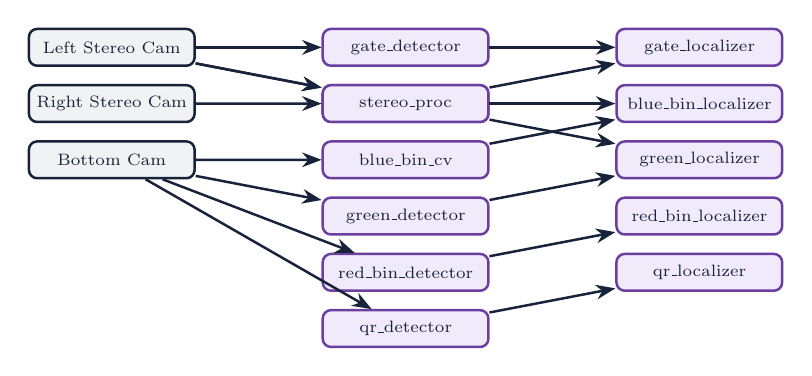
\begin{tikzpicture}[scale=0.85, every node/.append style={scale=0.85}, node distance=0.22cm and 0.5cm]
  \node[topobox,fill=ink!6,draw=ink] (lc) {Left Stereo Cam};
  \node[topobox,fill=ink!6,draw=ink, below=of lc] (rc) {Right Stereo Cam};
  \node[topobox,fill=ink!6,draw=ink, below=of rc] (bc) {Bottom Cam};

  \node[topobox, right=1.6cm of lc] (gd) {gate\_detector};
  \node[topobox, below=of gd] (bbd) {blue\_bin\_detector};
  \node[topobox, below=of bbd] (bbcv) {blue\_bin\_cv};
  \node[topobox, below=of bbcv] (grd) {green\_detector};
  \node[topobox, below=of grd] (rbd) {red\_bin\_detector};
  \node[topobox, below=of rbd] (qrd) {qr\_detector};
  \node[topobox, right=1.6cm of rc] (sp) {stereo\_proc};

  \node[topobox, right=1.6cm of gd] (gl) {gate\_localizer};
  \node[topobox, below=of gl] (bl) {blue\_bin\_localizer};
  \node[topobox, below=of bl] (grl) {green\_localizer};
  \node[topobox, below=of grl] (rbl) {red\_bin\_localizer};
  \node[topobox, below=of rbl] (qrl) {qr\_localizer};

  \draw[fsmarr] (lc) -- (gd);
  \draw[fsmarr] (lc) -- (bbd);
  \draw[fsmarr] (lc) -- (sp);
  \draw[fsmarr] (rc) -- (sp);
  \draw[fsmarr] (bc) -- (bbcv);
  \draw[fsmarr] (bc) -- (grd);
  \draw[fsmarr] (bc) -- (rbd);
  \draw[fsmarr] (bc) -- (qrd);
  \draw[fsmarr] (gd) -- (gl);
  \draw[fsmarr] (sp) -- (gl);
  \draw[fsmarr] (sp) -- (grl);
  \draw[fsmarr] (bbd) -- (bl);
  \draw[fsmarr] (bbcv) -- (bl);
  \draw[fsmarr] (grd) -- (grl);
  \draw[fsmarr] (rbd) -- (rbl);
  \draw[fsmarr] (qrd) -- (qrl);
\end{tikzpicture}
\caption{Fig 6. Perception Pipeline Topology: Optical Feeds to 3D Localizers}
\end{figure}

\begin{figure}[H]\centering
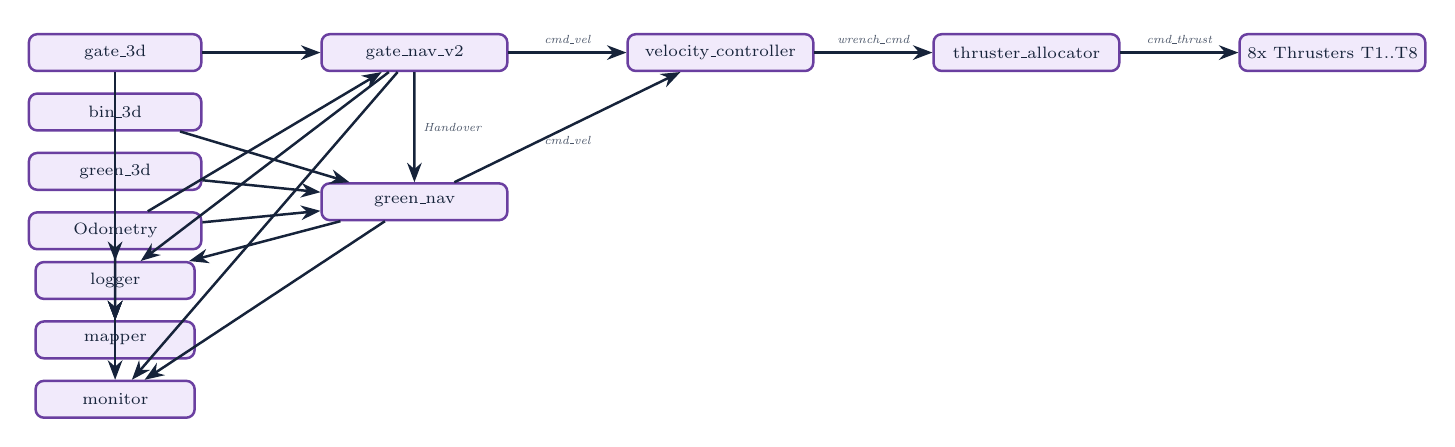
\begin{tikzpicture}[scale=0.85, every node/.append style={scale=0.85}, node distance=0.26cm and 0.7cm]
  \node[topobox,text width=2.4cm] (g3) {gate\_3d};
  \node[topobox,text width=2.4cm, below=of g3] (b3) {bin\_3d};
  \node[topobox,text width=2.4cm, below=of b3] (gr3) {green\_3d};
  \node[topobox,text width=2.4cm, below=of gr3] (od) {Odometry};

  \node[topobox,text width=2.6cm, right=1.5cm of g3] (gnv) {gate\_nav\_v2};
  \node[topobox,text width=2.6cm, below=1.4cm of gnv] (grn) {green\_nav};

  \node[topobox,text width=2.6cm, right=1.5cm of gnv] (vc) {velocity\_controller};
  \node[topobox,text width=2.6cm, right=1.5cm of vc] (ta) {thruster\_allocator};
  \node[topobox,text width=2.6cm, right=1.5cm of ta] (th) {8x Thrusters T1..T8};

  \node[topobox,text width=2.2cm, below=2.4cm of g3] (log) {logger};
  \node[topobox,text width=2.2cm, below=of log] (map) {mapper};
  \node[topobox,text width=2.2cm, below=of map] (mon) {monitor};

  \draw[fsmarr] (g3) -- (gnv);
  \draw[fsmarr] (b3) -- (grn);
  \draw[fsmarr] (gr3) -- (grn);
  \draw[fsmarr] (od) -- (gnv);
  \draw[fsmarr] (od) -- (grn);
  \draw[fsmarr] (gnv) -- node[above,fsmlabel]{cmd\_vel} (vc);
  \draw[fsmarr] (grn) -- node[below,fsmlabel]{cmd\_vel} (vc);
  \draw[fsmarr] (gnv) -- node[right,fsmlabel]{Handover} (grn);
  \draw[fsmarr] (vc) -- node[above,fsmlabel]{wrench\_cmd} (ta);
  \draw[fsmarr] (ta) -- node[above,fsmlabel]{cmd\_thrust} (th);
  \draw[fsmarr] (gnv) -- (log);
  \draw[fsmarr] (grn) -- (log);
  \draw[fsmarr] (od) -- (log);
  \draw[fsmarr] (od) -- (map);
  \draw[fsmarr] (g3) -- (map);
  \draw[fsmarr] (b3) -- (map);
  \draw[fsmarr] (gr3) -- (map);
  \draw[fsmarr] (od) -- (mon);
  \draw[fsmarr] (gnv) -- (mon);
  \draw[fsmarr] (grn) -- (mon);
\end{tikzpicture}
\caption{Fig 7. Planning, Closed-Loop Control, Thruster Allocation, and Telemetry Topology}
\end{figure}

\subsection{Comprehensive ROS 2 Topic \& Interface Catalog}

The table below details every active topic across the 10-package software stack, outlining
publishers, subscribers, message types, and functional roles:

\begin{table}[H]\centering\scriptsize
\begin{tabularx}{\textwidth}{L{4.4cm} L{2.6cm} L{3.0cm} X}
\toprule
\rowcolor{tablehead}\textbf{Topic Name} & \textbf{Publisher Node} & \textbf{Message Type} & \textbf{Data Content \& Role} \\
\midrule
\ttfamily .../stereo\_front/left/image\_raw & ros\_gz\_bridge & sensor\_msgs/Image & Left stereo 800$\times$600 optical feed for forward vision. \\
\ttfamily .../bottom/image\_raw & ros\_gz\_bridge & sensor\_msgs/Image & Downward camera stream for arena target inspection. \\
\ttfamily .../stereo\_front/disparity & stereo\_image\_proc & stereo\_msgs/DisparityImage & Dense disparity map for metric 3D depth computation. \\
\ttfamily /auv/gate\_detection\_2d & gate\_detector\_node & Float32MultiArray & Gate bounding box $[u,v,w,h,\text{conf}]$. \\
\ttfamily /auv/gate\_position\_3d & gate\_localizer\_node & Float32MultiArray & Gate 3D position $[x,y,z,\text{conf}]$ in vehicle body frame. \\
\ttfamily /auv/blue\_bin\_detection\_\newline bottom\_2d & blue\_bin\_cv\_detector & Float32MultiArray & 2D coordinates of blue drum satisfying green mat overlap. \\
\ttfamily /auv/blue\_bin\_position\_3d & blue\_bin\_localizer\_node & Float32MultiArray & 3D metric position of blue drum for visual centering. \\
\ttfamily /auv/green\_position\_3d & green\_localizer\_node & Float32MultiArray & 3D position of green landing mat centroid. \\
\ttfamily /auv/qr\_payload & qr\_detector\_node & std\_msgs/String & Decoded text payload from floor QR target cubes. \\
\ttfamily /auv/mission\_state & gate\_navigator\_v2\_node & std\_msgs/String & Active gate FSM state (FORWARD, TRACK, STOP, RETURN\_CROSS, DONE). \\
\ttfamily /auv/green\_mission\_state & green\_navigator\_node & std\_msgs/String & Post-gate FSM state (SEARCH\_GREEN, CENTER...). \\
\ttfamily /auv/forward\_reference\_yaw & gate\_navigator\_v2\_node & std\_msgs/Float32 & Locked reference heading (rad) for post-gate snap. \\
\ttfamily /model/auv\_box/cmd\_vel & gate\_navigator\_v2, green\_navigator & geometry\_msgs/Twist & Commanded body velocity: $v_x$ (surge), $v_y$ (sway), $\omega_z$ (yaw). \\
\ttfamily /auv/wrench\_cmd & velocity\_controller\_node & geometry\_msgs/Wrench & Net body wrench $[F_x,F_y,F_z,M_x,M_y,M_z]$. \\
\ttfamily /model/auv\_box/joint/\newline T\_\{1..8\}/cmd\_thrust & thruster\_allocator\_node & std\_msgs/Float64 & Newton thrust commands distributed across 8 thrusters. \\
\ttfamily /auv/odom & ros\_gz\_bridge & nav\_msgs/Odometry & Ground-truth vehicle odometry and orientation. \\
\ttfamily /odometry/filtered & robot\_localization (EKF) & nav\_msgs/Odometry & Fused, drift-free state estimate from IMU + Odometry. \\
\ttfamily /auv/trail\_map & trail\_mapper\_node & nav\_msgs/Path & Full 3D mission trajectory history path. \\
\bottomrule
\end{tabularx}
\end{table}

%% ============================================================
\section{Mission Telemetry \& Mapping}

During each mission, the AUV actively tracks its trajectory. The \hl{trail\_mapper\_node}
records the AUV's odometry at 1Hz, along with the precise 3D locations of the detected
obstacles, generating a comprehensive top-down spatial footprint at shutdown. In parallel,
\hl{mission\_logger\_node} writes a 30+ column CSV capturing all vehicle dynamics, while
\hl{mission\_monitor\_node} provides a live ANSI terminal dashboard.

\begin{figure}[H]\centering
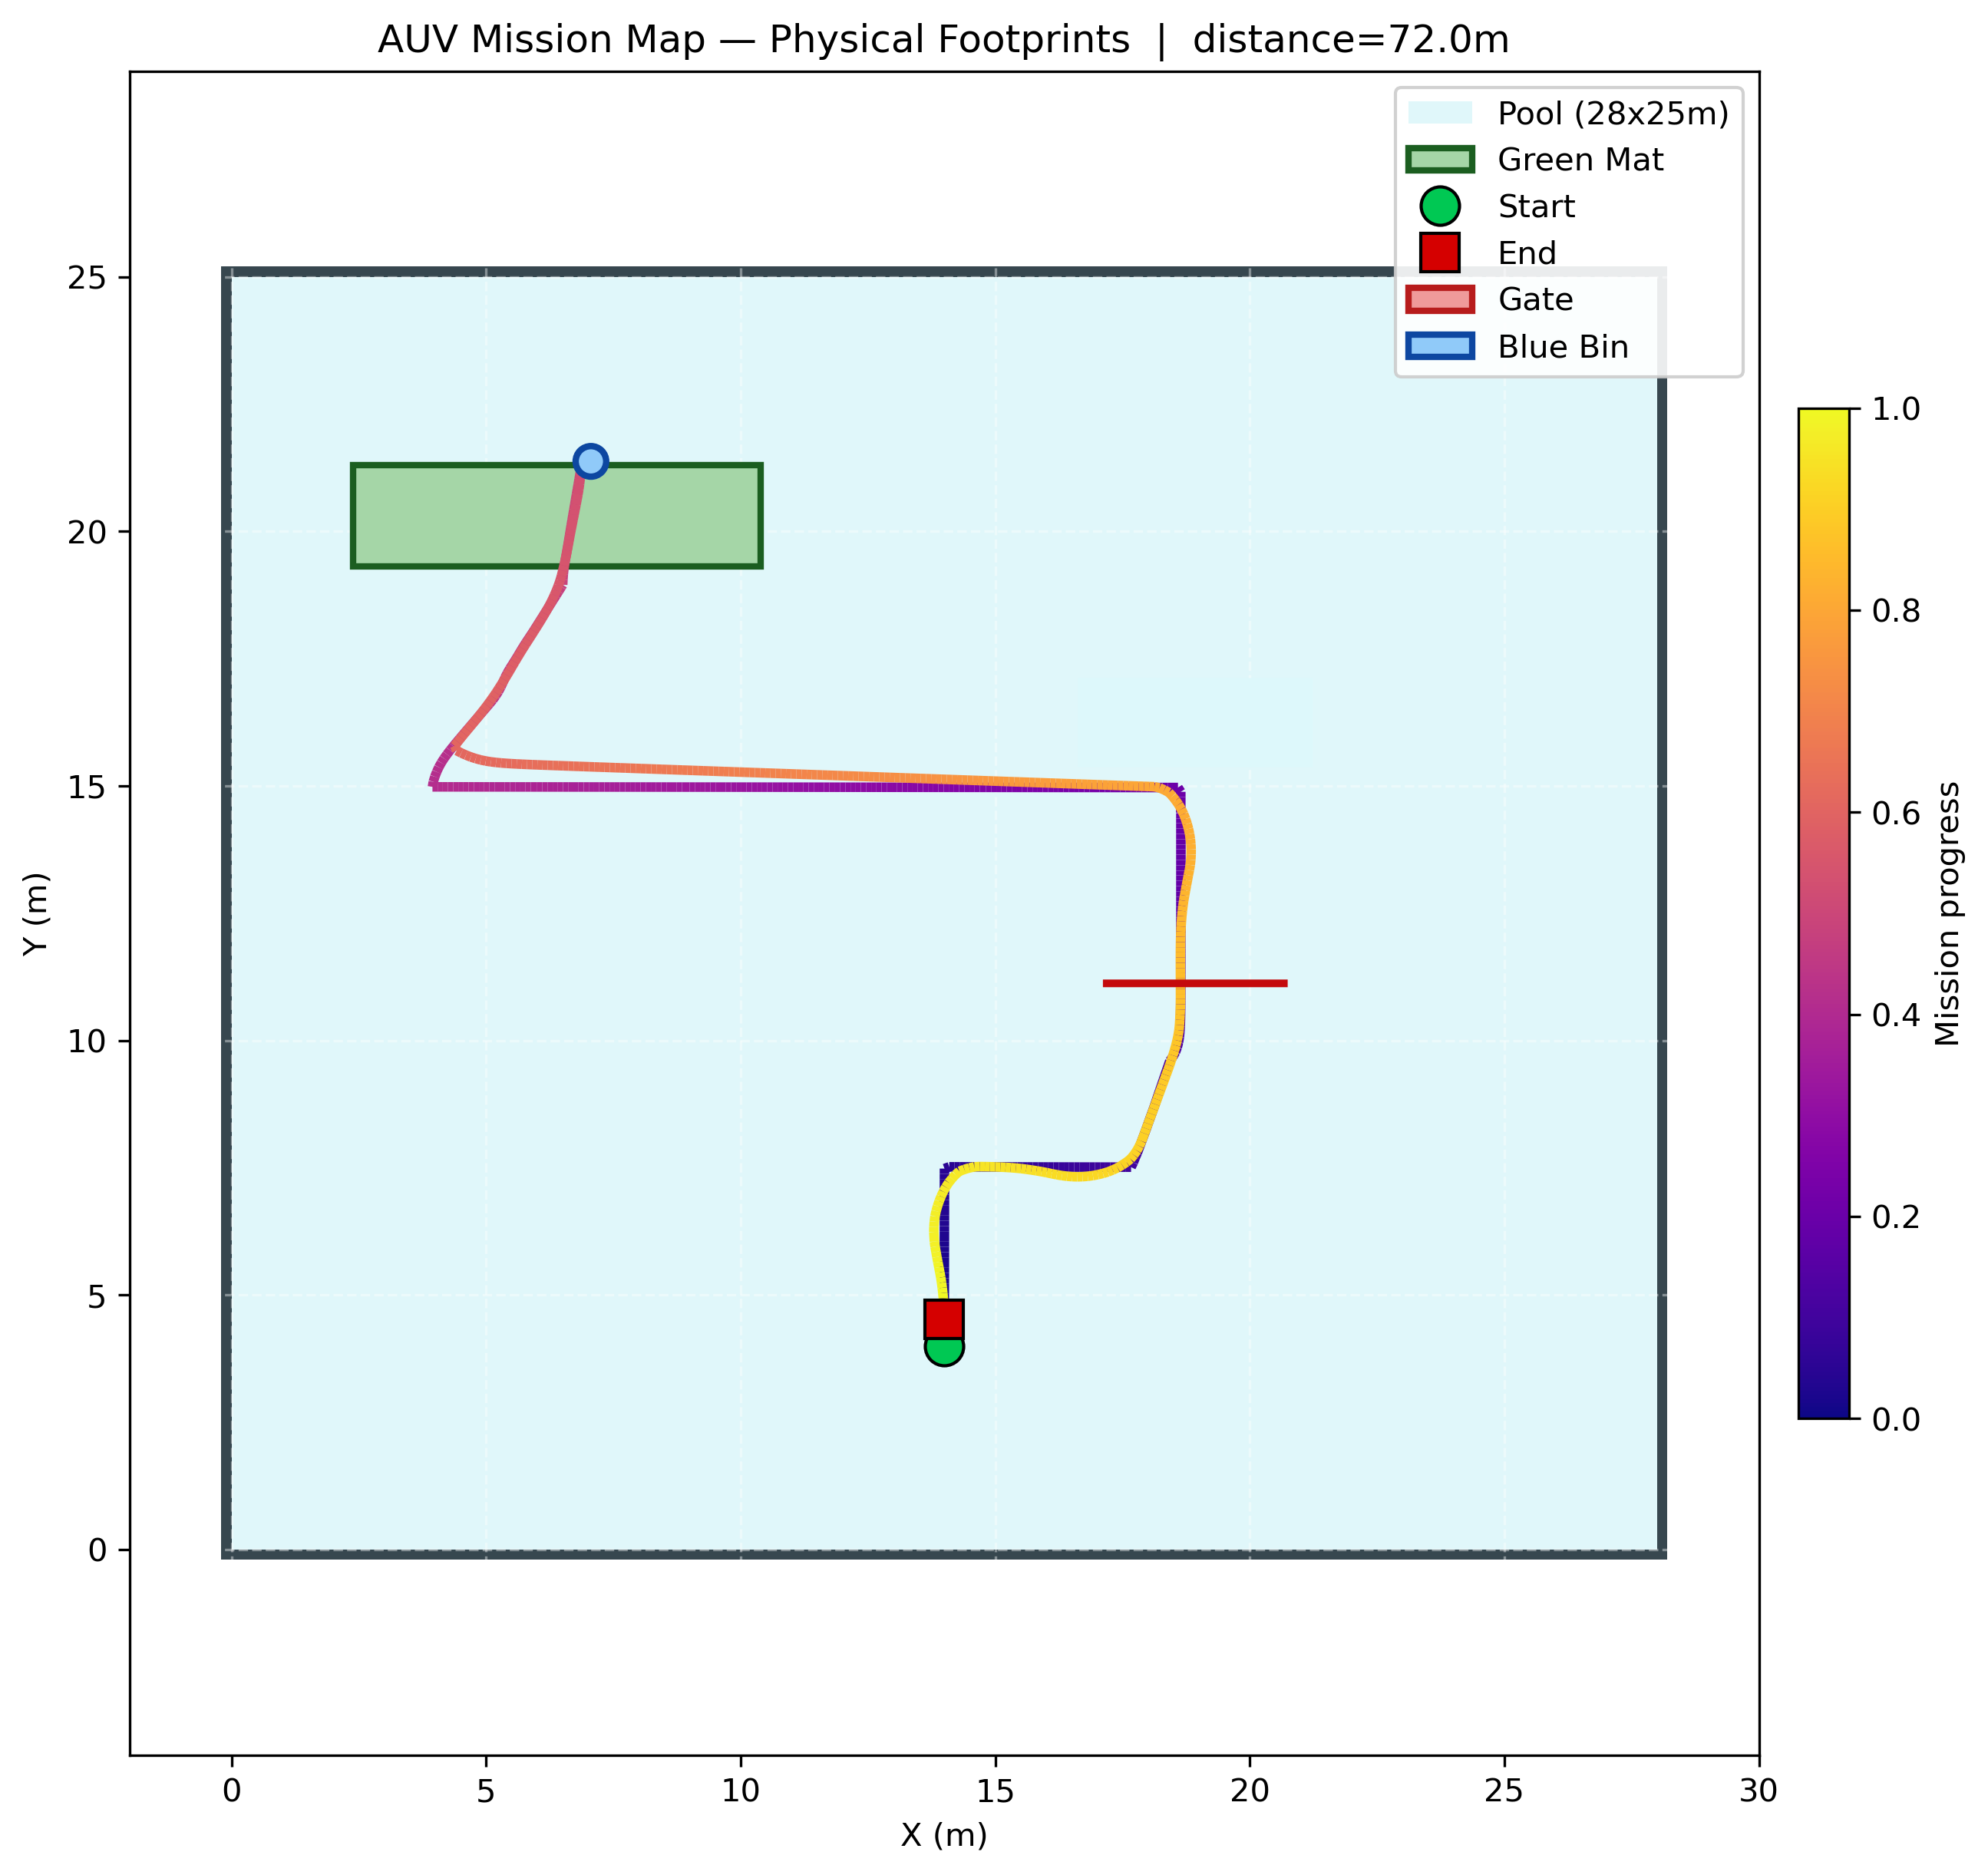
\includegraphics[width=0.8\textwidth]{photos_v2/fig8_mission_map_retrace.png}
\caption{Fig 8. Auto-Generated 2D Mission Trajectory Map (distance = 72.0m) Showing the Gate
Crossing, Lateral Traverse Along the Arena, and Approach to the Green Mat / Blue Bin.}
\end{figure}

\end{document}
